\chapter{Discussão dos Resultados}
\label{chap:discussao}

\subsection{Discussão dos Resultados da Simulação}

Para a geração dos cenários de simulação, estabeleceram-se diferentes configurações para os parâmetros cognitivos e operacionais do trabalhador (\textit{TrainingCycles}, \textit{ProductionCycles}, \textit{InspectionCycles}, \textit{FeedbackCycles} e \textit{StressCycles}). Durante as rodadas de testes, os fatores de influência variaram em uma escala de 1 a 10, com exceção do parâmetro \textit{ProductionCycles}, cujo domínio de variação foi de 1 a 100.O incremento numérico desses parâmetros representa uma melhoria progressiva nas condições do trabalhador, exceto para o \textit{StressCycles}, que possui uma correlação inversamente proporcional: o valor 1 representa uma condição de estresse máximo, enquanto o valor 10 indica uma condição totalmente livre de estresse.

A partir da execução do modelo, foram extraídas métricas de controle de qualidade para avaliar o comportamento do sistema. O primeiro cenário-base foi simulado atribuindo-se o valor mínimo unitário a todos os parâmetros de influência, configurando um ambiente caracterizado por alta pressão, baixa experiência e elevado nível de fadiga. A Figura \ref{fig:conformidadep1} ilustra o número de conformidades por fôrma, ou seja, a quantidade de ciclos completos de montagem executados sem a omissão de nenhuma atividade obrigatória.

\begin{figure}[!htb]
	\centering
	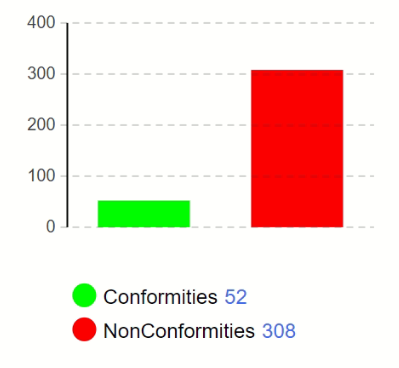
\includegraphics[width=0.6\linewidth]{Caps/Figs/conformidadeP1}
	\caption{Resultado das conformidades globais por fôrma com todos os fatores de influência no valor mínimo (1).}
	\fonte{Autoral.}
	\label{fig:conformidadep1}
\end{figure}
\FloatBarrier

A análise deste cenário revela um elevado índice de desvios comportamentais na linha de produção simulada. O modelo registrou apenas 52 conformidades globais (\textit{Conformities}) em comparação com 308 não conformidades (\textit{NonConformities}). Esse resultado evidencia que condições operacionais adversas impactam diretamente a tomada de decisão do trabalhador, aumentando a probabilidade de omissão de etapas durante a execução das atividades.

A Figura \ref{fig:conformidadeatividadep1} apresenta o volume de conformidades contabilizadas individualmente por atividade. Diferentemente da métrica global por fôrma, este indicador contabiliza todas as tarefas executadas corretamente (\textit{ConformitiesPerActivity}) em relação ao total de tarefas negligenciadas (\textit{NonConformitiesPerActivity}) ao longo de toda a simulação.

\begin{figure}[!htb]
	\centering
	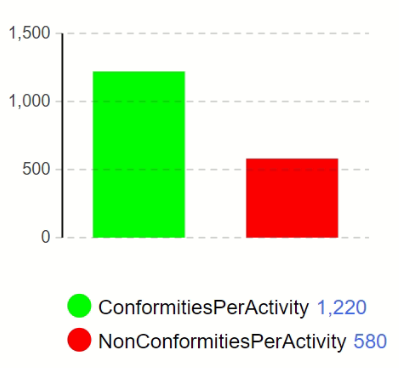
\includegraphics[width=0.6\linewidth]{Caps/Figs/conformidadeAtividadeP1}
	\caption{Resultado das conformidades por atividade com todos os fatores de influência no valor mínimo (1).}
	\fonte{Autoral.}
	\label{fig:conformidadeatividadep1}
\end{figure}
\FloatBarrier

Foram observadas 1220 atividades executadas conforme o padrão estabelecido e 580 atividades negligenciadas. Nota-se, portanto, uma diferença significativa entre o número de não conformidades globais e o número de não conformidades por atividade. Embora o trabalhador não negligencie todas as etapas do processo, basta que uma única atividade seja ignorada em um ciclo de montagem ou desmontagem para que toda a execução daquela fôrma seja classificada como não conforme.

A Figura \ref{fig:conformidadepizzap1} destaca a distribuição percentual das atividades ignoradas durante a execução das tarefas.

\begin{figure}[!htb]
	\centering
	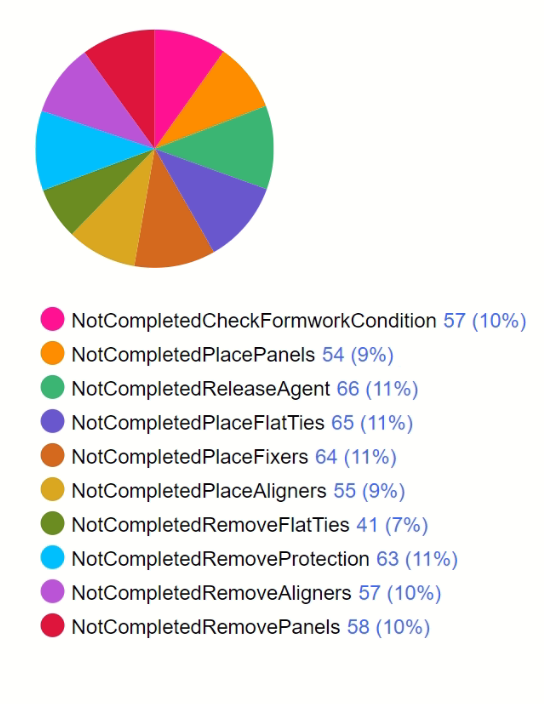
\includegraphics[width=0.7\linewidth]{Caps/Figs/conformidadePizzaP1}
	\caption{Porcentagem de tarefas ignoradas durante o processo para os parâmetros mínimos.}
	\fonte{Autoral.}
	\label{fig:conformidadepizzap1}
\end{figure}
\FloatBarrier

Observa-se uma baixa variação percentual entre as tarefas ignoradas, indicando que o trabalhador não apresenta tendência significativa de negligenciar uma atividade específica em relação às demais. Dessa forma, o comportamento inadequado distribui-se de maneira relativamente uniforme entre as etapas do processo.

Em seguida, realizou-se a análise do cenário com todos os parâmetros de influência configurados em seus valores máximos.

\begin{figure}[!htb]
	\centering
	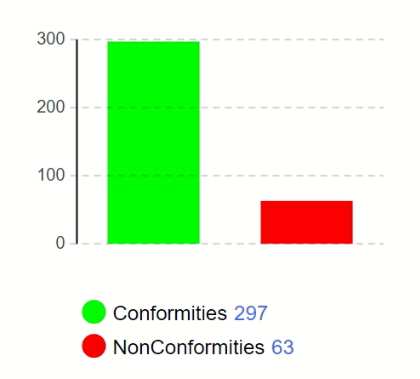
\includegraphics[width=0.6\linewidth]{Caps/Figs/conformidadep2}
	\caption{Resultado das conformidades globais por fôrma com todos os fatores de influência no valor máximo.}
	\fonte{Autoral.}
	\label{fig:conformidadep2}
\end{figure}
\FloatBarrier

A análise deste cenário revela uma redução significativa no índice de desvios comportamentais da linha de produção simulada. O modelo registrou 297 conformidades globais (\textit{Conformities}) e apenas 63 não conformidades (\textit{NonConformities}). Esse resultado demonstra que a melhoria dos parâmetros de influência impacta positivamente o comportamento do trabalhador, reduzindo a probabilidade de omissão de atividades durante o processo.

A Figura \ref{fig:conformidadeatividadep2} apresenta o volume de conformidades contabilizadas individualmente por atividade para o cenário com parâmetros máximos.

\begin{figure}[!htb]
	\centering
	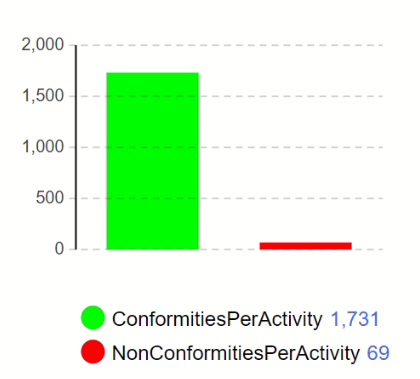
\includegraphics[width=0.6\linewidth]{Caps/Figs/conformidadeatividadep2}
	\caption{Resultado das conformidades por atividade com todos os fatores de influência no valor máximo.}
	\fonte{Autoral.}
	\label{fig:conformidadeatividadep2}
\end{figure}
\FloatBarrier

Foram observadas 1731 atividades executadas conforme o padrão e apenas 69 atividades negligenciadas. Em comparação com os resultados apresentados na Figura \ref{fig:conformidadeatividadep1}, verifica-se uma redução significativa na quantidade de atividades ignoradas, correspondente a aproximadamente 88,10\%.

\begin{figure}[!htb]
	\centering
	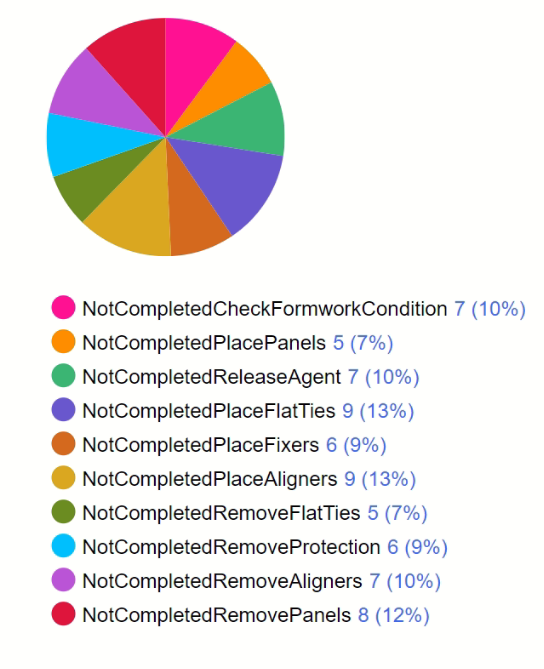
\includegraphics[width=0.7\linewidth]{Caps/Figs/conformidadepizzap2}
	\caption{Porcentagem de tarefas ignoradas durante o processo para os parâmetros máximos.}
	\fonte{Autoral.}
	\label{fig:conformidadepizzap2}
\end{figure}
\FloatBarrier

A análise da Figura \ref{fig:conformidadepizzap2} demonstra que as atividades negligenciadas permaneceram distribuídas de forma relativamente uniforme entre as diferentes etapas do processo, indicando que a melhoria dos fatores de influência reduziu globalmente a ocorrência de falhas, sem concentrar o comportamento inadequado em uma atividade específica.

Ademais, a fim de ampliar as possibilidades de análise da simulação, o AnyLogic disponibiliza diferentes ferramentas experimentais, tais como \textit{Parameter Variation}, \textit{Optimization}, \textit{Monte Carlo}, \textit{Calibration}, \textit{Reinforcement Learning (RL)}, \textit{Compare Runs} e \textit{Sensitivity Analysis} . Neste estudo, utilizaremos \textit{Compare Runs} e \textit{Sensitivity Analysis}.

O experimento \textit{Compare Runs} (Comparar Execuções) permite executar o modelo de simulação múltiplas vezes utilizando diferentes configurações de parâmetros, facilitando a comparação visual e quantitativa entre os resultados obtidos.

Para a análise dos resultados deste trabalho, foi realizado um experimento variando os parâmetros de influência e observando seu impacto na probabilidade de o trabalhador ignorar uma etapa do processo. Foram definidos cinco cenários experimentais:

\begin{itemize}
	\item[a)] Todos os fatores de influência com valor 1;
	\item[b)] Todos os fatores de influência com valor 1 e \textit{WorkerTrainingCycles} com valor 5;
	\item[c)] Todos os fatores de influência com valor 1 e \textit{WorkerTrainingCycles} com valor 10;
	\item[d)] Todos os fatores de influência com valor 1, \textit{WorkerTrainingCycles} com valor 10 e \textit{WorkerProductionCycles} com valor 5;
	\item[e)] Todos os fatores de influência com valor 1, \textit{WorkerTrainingCycles} com valor 10 e \textit{WorkerProductionCycles} com valor 10.
\end{itemize}

\begin{figure}[!htb]
	\centering
	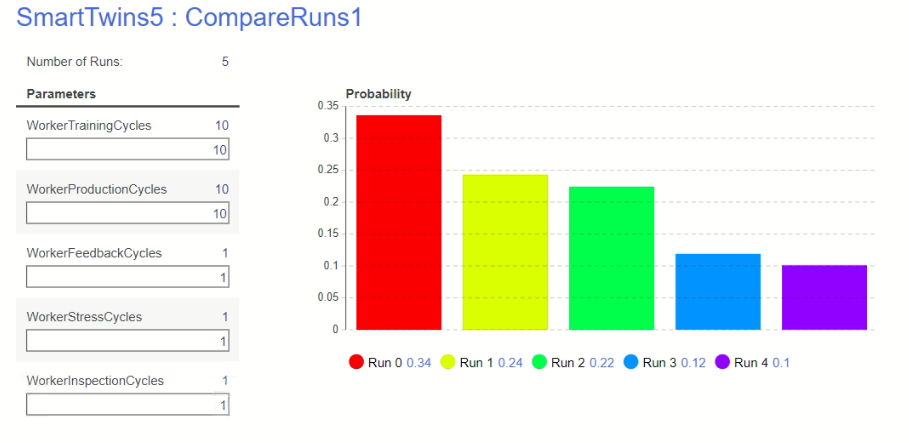
\includegraphics[width=0.7\linewidth]{Caps/Figs/compareruns}
	\caption{Resultado do experimento \textit{Compare Runs} para os cinco cenários analisados.}
	\fonte{Autoral.}
	\label{fig:compareruns}
\end{figure}
\FloatBarrier

Os resultados obtidos demonstraram uma redução progressiva na probabilidade de o trabalhador ignorar etapas à medida que os parâmetros de influência foram aumentados. No cenário (a), a probabilidade observada foi de 0,34. Ao aumentar apenas o parâmetro \textit{WorkerTrainingCycles} para 5 no cenário (b), a probabilidade reduziu para 0,24, representando uma diminuição aproximada de 29,41\% em relação ao cenário inicial.

No cenário (c), ao elevar \textit{WorkerTrainingCycles} para 10, a probabilidade passou para 0,22, correspondendo a uma redução adicional de apenas 8,33\% em relação ao cenário (b). Esse comportamento indica que o aumento isolado de um único parâmetro tende a apresentar retornos decrescentes na melhoria do desempenho cognitivo do trabalhador.

Por outro lado, ao combinar o aumento de diferentes fatores de influência, os resultados apresentaram reduções significativamente mais expressivas. No cenário (d), ao manter \textit{WorkerTrainingCycles} em 10 e elevar \textit{WorkerProductionCycles} para 5, a probabilidade caiu para 0,12, representando uma redução de aproximadamente 45,45\% em relação ao cenário (c).

Por fim, no cenário (e), com ambos os parâmetros \textit{WorkerTrainingCycles} e \textit{WorkerProductionCycles} configurados com valor 10, a probabilidade foi reduzida para 0,10, alcançando uma redução total de aproximadamente 70,59\% em relação ao cenário-base.

Os resultados sugerem que o aumento conjunto dos fatores de influência apresenta maior efetividade na redução das falhas cognitivas do que o aumento isolado de apenas um parâmetro específico. Dessa forma, o modelo evidencia que melhorias simultâneas em treinamento, experiência e demais fatores humanos possuem impacto mais significativo na redução da probabilidade de omissão de atividades durante o processo produtivo.

O experimento de \textit{Sensitivity Analysis} (Análise de Sensibilidade) é utilizado para avaliar como alterações em parâmetros de entrada impactam os resultados finais da simulação. Nesse tipo de experimento, o modelo é executado múltiplas vezes variando-se apenas um parâmetro por vez, permitindo analisar individualmente sua influência sobre as variáveis de saída.

Foram definidos dois cenários experimentais:

\begin{itemize}
	\item[a)] Parâmetros configurados com valor mínimo e variação do \textit{WorkerTrainingCycles} de 1 a 10 em relação à probabilidade de ignorar etapas;
	\item[b)] Parâmetros configurados com valor mínimo e variação do \textit{WorkerProductionCycles} de 1 a 10 em relação à probabilidade de ignorar etapas.
\end{itemize}

\begin{figure}[!htb]
	\centering
	\caption{Resultados da \textit{Sensitivity Analysis} para os cenários analisados.}
	
	\begin{minipage}{0.5\textwidth}
		\centering
		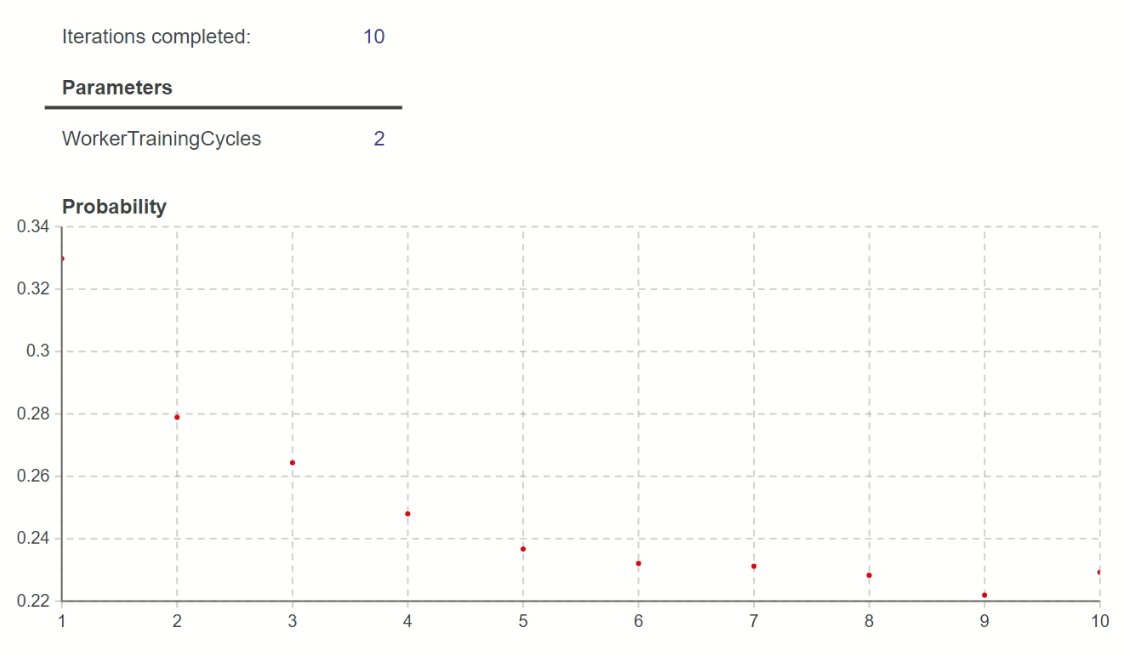
\includegraphics[width=\textwidth]{Caps/Figs/trainingsensitivity.png}
		\label{fig:trainingsensitivity}
	\end{minipage}
	\hfill
	\begin{minipage}{0.5\textwidth}
		\centering
		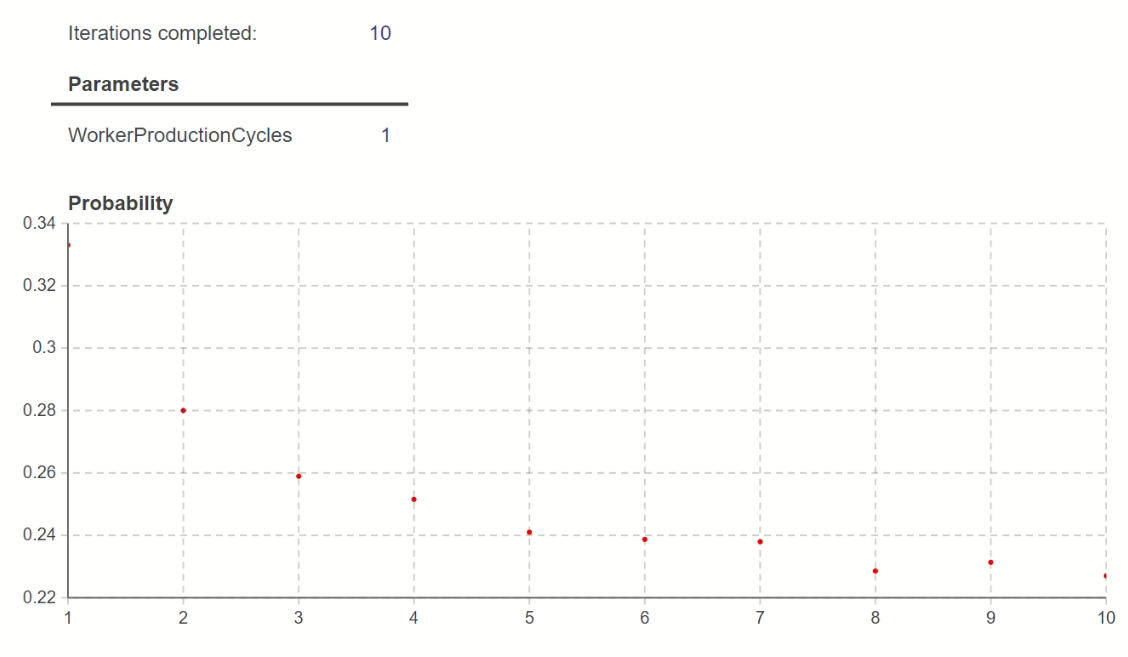
\includegraphics[width=\textwidth]{Caps/Figs/productionsensitivity.png}
		\label{fig:productionsensitivity}
	\end{minipage}
	
	\fonte{Autoral.}
	
\end{figure}
\FloatBarrier

A análise da Figura \ref{fig:trainingsensitivity} demonstra que os valores iniciais de probabilidade apresentam comportamento semelhante para ambos os cenários, iniciando próximos de 0,34 e 0,32. À medida que os parâmetros aumentam, observa-se uma tendência de decaimento exponencial da probabilidade de ignorar etapas, indicando que o crescimento dos fatores de influência reduz progressivamente a ocorrência de falhas cognitivas no processo.

Além disso, os gráficos apresentam comportamentos bastante semelhantes entre si, sugerindo que, para os parâmetros analisados, não há evidências de que um fator exerça influência significativamente superior ao outro sobre a redução da probabilidade de omissão de atividades. Dessa forma, os resultados indicam que tanto o aumento do treinamento quanto o aumento da experiência produtiva contribuem de maneira consistente para a melhoria do desempenho do trabalhador no modelo proposto.

Embora a análise tenha sido realizada apenas para os parâmetros \textit{WorkerTrainingCycles} e \textit{WorkerProductionCycles}, os resultados sugerem que os fatores de influência possuem comportamento semelhante dentro da formulação adotada no modelo.

\subsection{Discussão dos Resultados do Autômato Diagnosticador $G_d$}

Como discutido na Revisão da Literatura, na Seção \ref{subsec:diagnosticabilidade}, a construção do Autômato Diagnosticador $G_d$ por si só não garante que o sistema seja Diagnosticável. Para que um sistema seja considerado Diagnosticável, é necessário que, após a ocorrência de uma falha, exista um número finito de Eventos Observáveis capaz de permitir a identificação inequívoca da falha ocorrida.

Por outro lado, um sistema é classificado como Não Diagnosticável quando o autômato Diagnosticador permanece em estados de incerteza, nos quais não é possível distinguir se o sistema se encontra em condição normal ou em condição de falha apenas pela observação dos eventos disponíveis. Em outras palavras, um sistema é Diagnosticável quando, nos estados finais do Diagnosticador $G_d$, torna-se possível diferenciar claramente estados rotulados como normais daqueles rotulados como falha.

A partir do Autômato Diagnosticador apresentado na Figura \ref{fig:diagnosticador}, foram analisados os estados finais do sistema, conforme ilustrado na Figura \ref{fig:diagnosticadorestadosfinais}.

\begin{figure}[!htb]
	\centering
	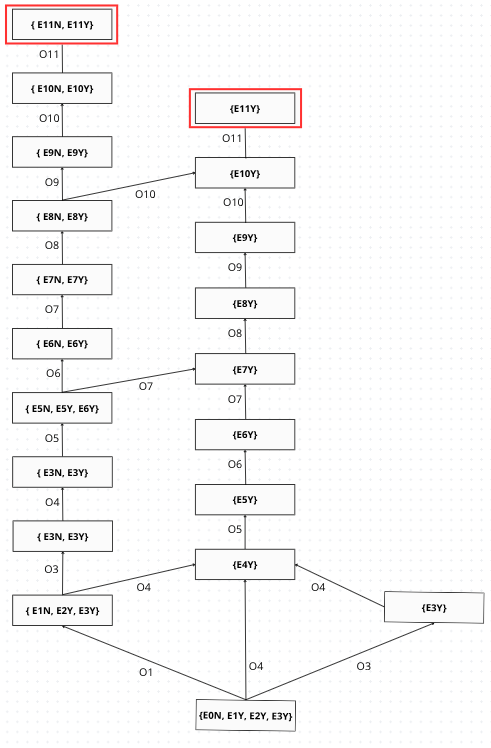
\includegraphics[width=0.7\linewidth]{Caps/Figs/diagnosticadorEstadosFinais}
	\caption{Estados finais do Autômato Diagnosticador.}
	\fonte{Autoral.}
	\label{fig:diagnosticadorestadosfinais}
\end{figure}
\FloatBarrier

Os estados finais do Diagnosticador $G_d$ correspondem ao estado de incerteza com $E11$ rotulado como $N$ (normal) e $E11$ rotulado como $Y$ (falha) e ao estado com $E11$ rotulado como $Y$ (falha). Dessa forma, verifica-se que o sistema modelado é \textbf{Não Diagnosticável}.

Isso significa que, analisando apenas os eventos observáveis disponíveis no sistema, um gestor ou sistema de supervisão não conseguiria determinar com exatidão se determinadas atividades foram realmente executadas ou se alguma falha ocorreu durante o processo. Em termos práticos, o sistema pode evoluir para o mesmo estado operacional independentemente da ocorrência de falhas, produzindo sequências observáveis indistinguíveis.


A não diagnosticabilidade observada está diretamente relacionada à existência de eventos não observáveis e às trajetórias paralelas geradas pelas transições de falha no autômato original. 

\subsubsection{Análise de cenário}Para uma análise mais detalhada da diagnosticabilidade do sistema, foi construído um novo cenário para o Autômato Diagnosticador. Nesse cenário, em vez de considerar a entrada $U_1$ (omissão da verificação das condições iniciais) como um evento não observável, supõe-se que essa etapa possa ser monitorada e identificada pelo sistema supervisor, passando então a ser tratada como um Evento Observável, denominado $O_2$.

A partir dessa modificação, um novo autômato $G$ foi gerado, conforme apresentado na Figura \ref{fig:automatogcenario}.

\begin{figure}[!htb]
	\centering
	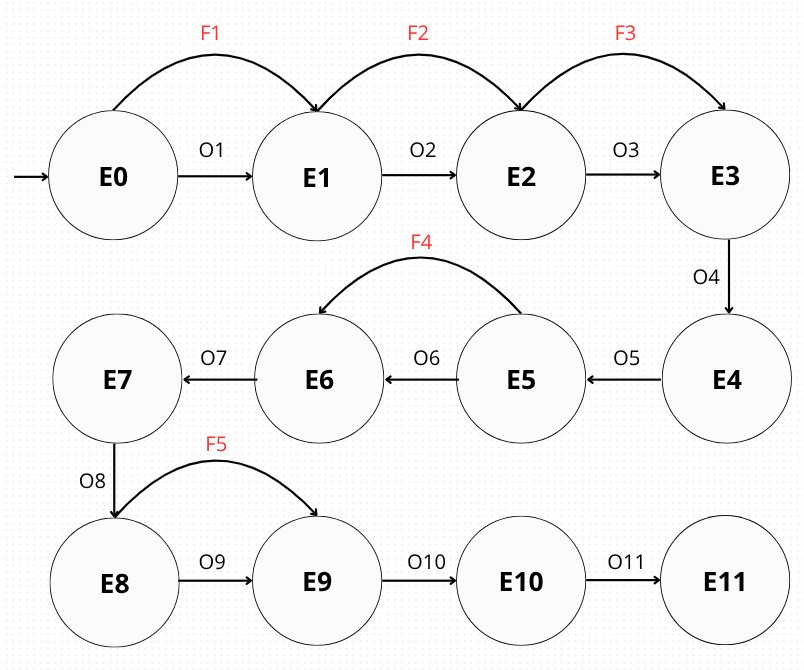
\includegraphics[width=0.7\linewidth]{Caps/Figs/automatoGcenario}
	\caption{Cenário modificado do autômato $G$.}
	\fonte{Autoral.}
	\label{fig:automatogcenario}
\end{figure}
\FloatBarrier

Com a alteração da observabilidade do evento associado à omissão da verificação inicial, foi realizada novamente a composição paralela entre o autômato do sistema $G$ e o autômato rotulador $G_{Al}$. O resultado dessa composição pode ser observado na Figura \ref{fig:resultadocomposicaoparalelacenario}.

\begin{figure}[!htb]
	\centering
	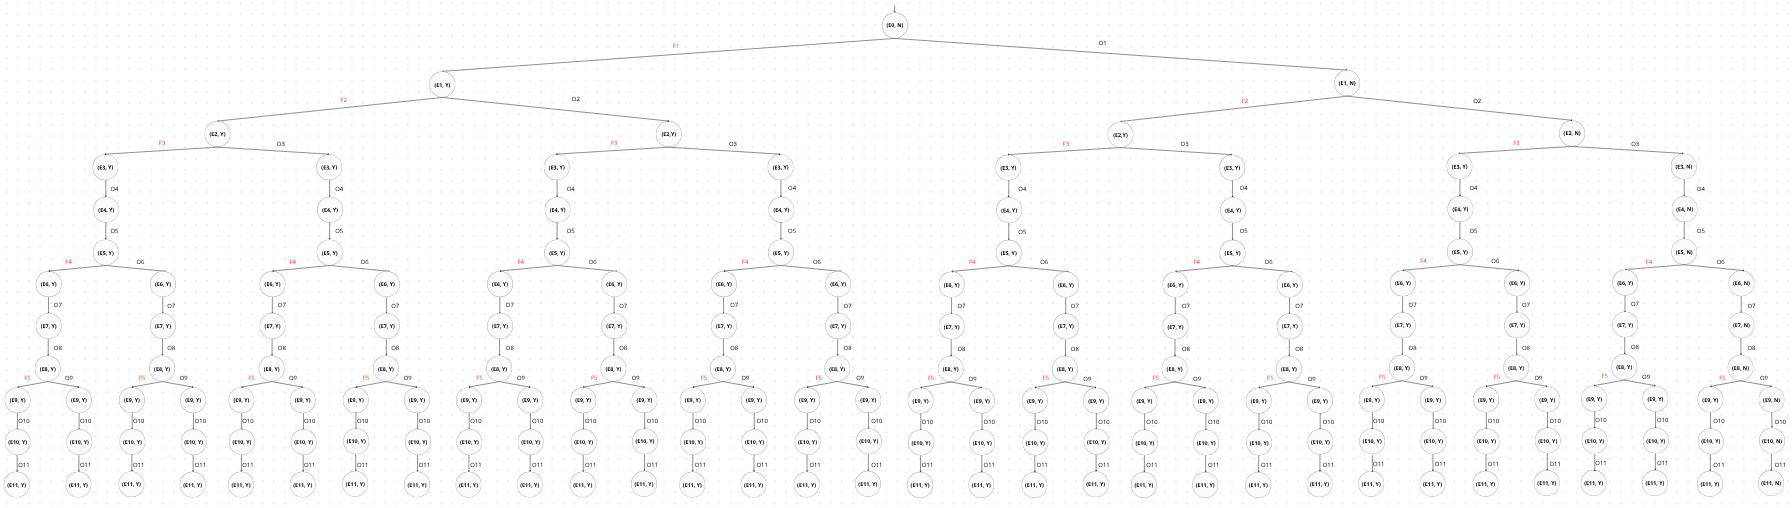
\includegraphics[width=1\linewidth]{Caps/Figs/resultadocomposicaoparalelaCenario}
	\caption{Resultado global da composição paralela para o cenário modificado.}
	\fonte{Autoral.}
	\label{fig:resultadocomposicaoparalelacenario}
\end{figure}

\begin{figure}[!htb]
	\centering
	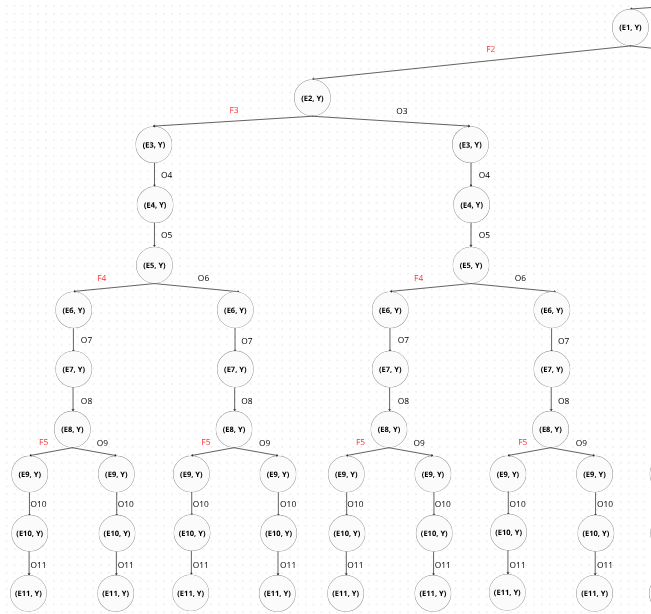
\includegraphics[width=\linewidth]{Caps/Figs/resultadocomposicaoparalelacenariop1}
	
	\caption{Resultado da composição paralela do cenário modificado (Parte 1).}
	\fonte{Autoral.}
	\label{fig:resultadocomposicaoparalelacenario1}
\end{figure}

\FloatBarrier
\clearpage

\begin{figure}[!htb]
	\ContinuedFloat
	\centering
	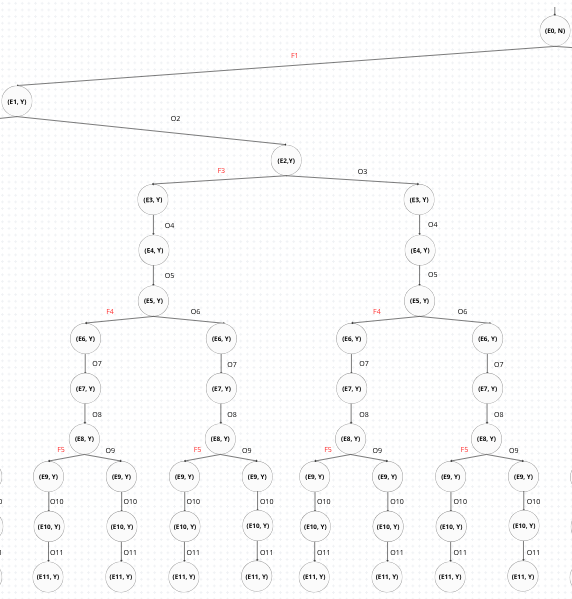
\includegraphics[width=\linewidth]{Caps/Figs/resultadocomposicaoparalelacenariop2}
	
	\caption{Resultado da composição paralela do cenário modificado (Parte 2).}
\end{figure}

\FloatBarrier
\clearpage

\begin{figure}[!htb]
	\ContinuedFloat
	\centering
	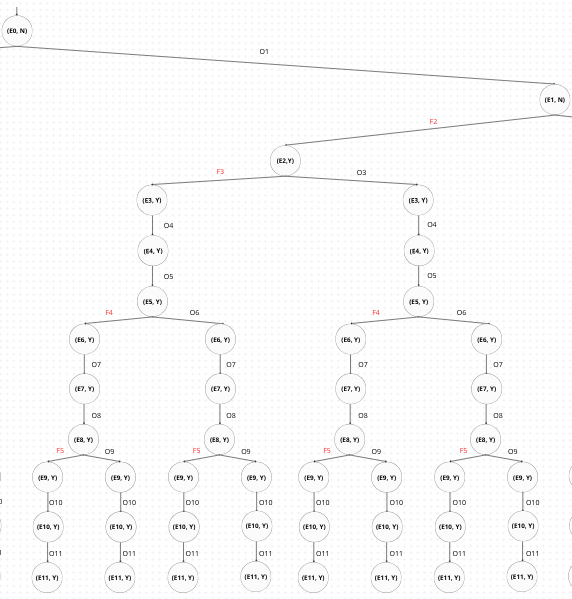
\includegraphics[width=\linewidth]{Caps/Figs/resultadocomposicaoparalelacenariop3}
	
	\caption{Resultado da composição paralela do cenário modificado (Parte 3).}
\end{figure}

\FloatBarrier
\clearpage

\begin{figure}[!htb]
	\ContinuedFloat
	\centering
	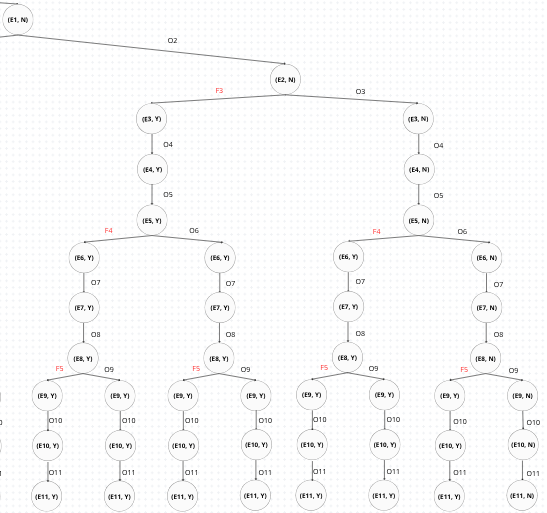
\includegraphics[width=\linewidth]{Caps/Figs/resultadocomposicaoparalelacenariop4}
	
	\caption{Resultado da composição paralela do cenário modificado (Parte 4).}
\end{figure}

\FloatBarrier

Após a aplicação do operador observador sobre a Composição Paralela, foi obtido o novo Autômato Diagnosticador apresentado na Figura \ref{fig:diagnosticadorCenario}.

\begin{figure}[!htb]
	\centering
	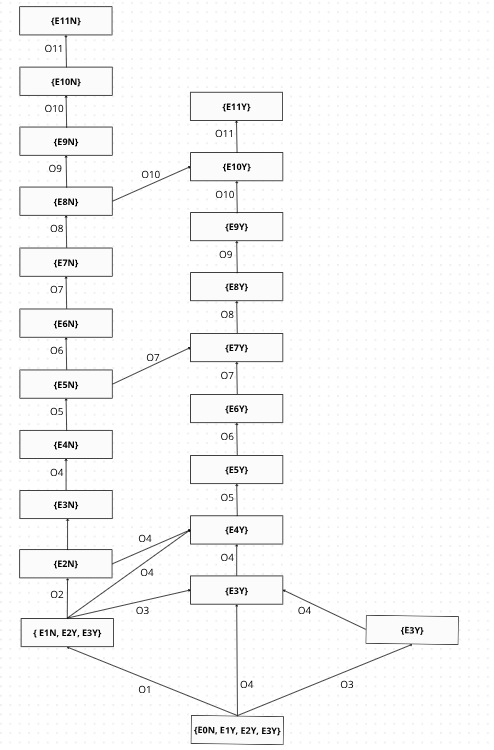
\includegraphics[width=0.7\linewidth]{Caps/Figs/diagnosticadorCenario}
	\caption{Autômato Diagnosticador do cenário modificado.}
	\fonte{Autoral.}
	\label{fig:diagnosticadorCenario}
\end{figure}
\FloatBarrier

A análise dos estados finais do novo diagnosticador demonstra que o sistema passa a apresentar comportamento \textbf{Diagnosticável}. Nesse cenário, os estados finais permitem distinguir claramente entre o estado $E_{11}$ rotulado como $N$ (normal) e o estado $E_{11}$ rotulado como $Y$ (falha), eliminando a ambiguidade presente no modelo anterior.

Dessa forma, conclui-se que a observabilidade do evento associado à omissão da verificação das condições iniciais é determinante para a Diagnosticabilidade do sistema. Quando essa etapa passa a ser monitorada explicitamente, o Diagnosticador consegue identificar em tempo finito a ocorrência da falha, tornando possível diferenciar trajetórias normais de trajetórias com falha.




